\begin{problem}{진흥이의 쌀 배달}{standard input}{standard output}{2 seconds}{1024 megabytes}

진흥이가 살고 있는 도시는 $N$개의 마을로 이루어져 있으며, 이 마을들은 트리 구조로 도로가 연결되어 있습니다. 트리는 사이클이 없는 연결 그래프를 말합니다. 따라서 임의의 두 마을 사이에는 오직 하나의 경로만 존재합니다.

도시의 중심에는 $0$번 마을이 있는데, 이곳은 모든 쌀을 모아두는 중앙 창고의 역할을 합니다. 나머지 $1$번부터 $N$번 마을까지는 각각 쌀을 생산하는 생산지입니다.

진흥이는 각 생산지를 방문해 그곳에서 생산된 쌀포대를 수거하여 $0$번 마을의 중앙 창고로 운반해야 합니다. 하지만 진흥이가 한 번에 옮길 수 있는 양에는 한계가 있어, 한 번 이동할 때 최대 $K$개의 쌀포대만 운반할 수 있습니다. 따라서 어떤 마을의 쌀포대를 모두 옮기려면 여러 번 오가야 할 수도 있습니다. \textbf{또한, 진흥이는 운반 중인 쌀포대를 잠시 다른 마을에 내려놓을 수도 있습니다.}

각 마을 $i$에는 $s_i$개의 쌀포대가 있으며, 각 도로마다 이동하는 데 걸리는 시간이 분 단위로 주어집니다. 진흥이는 처음에 중앙 창고가 있는 $0$번 마을에서 출발합니다. 쌀포대를 수거하거나 창고에 내려놓는 데 걸리는 시간은 없다고 가정합니다.

\begin{center}
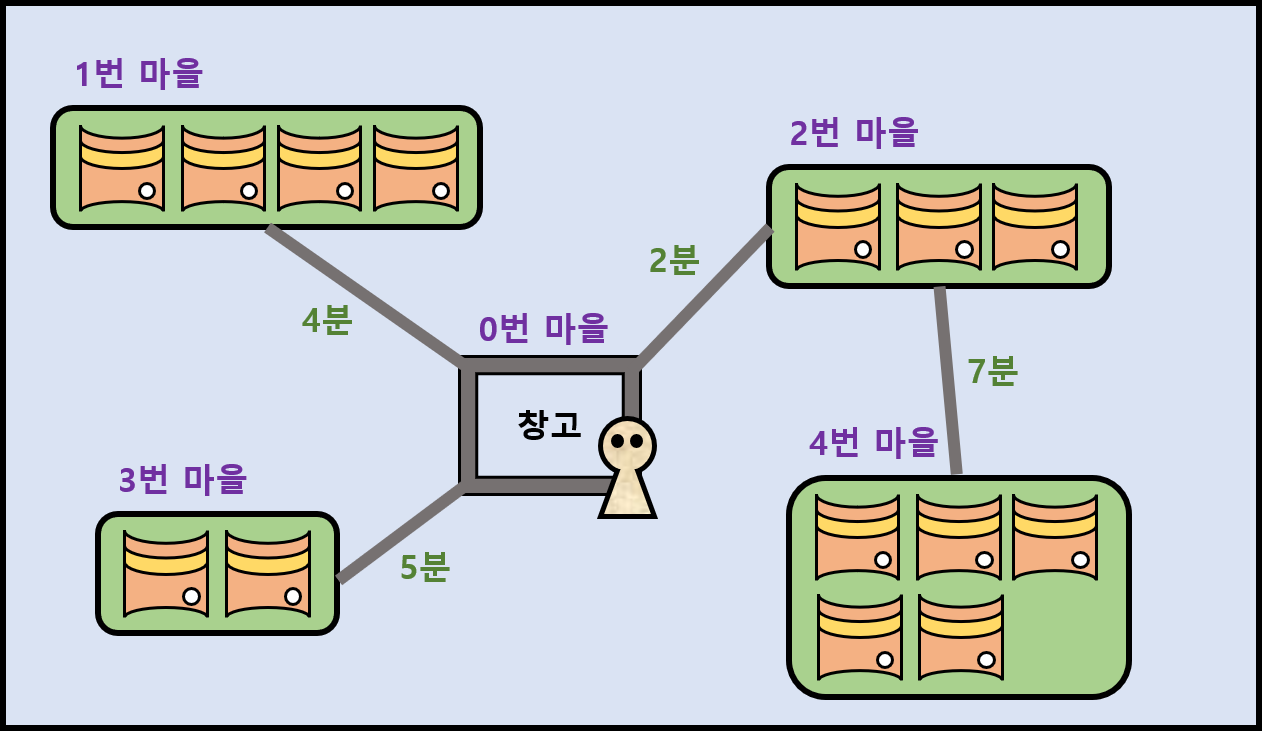
\includegraphics{town.png}
\end{center}

진흥이가 임무를 완수하기 위해 필요한 최소 시간을 분 단위로 출력하세요.

\InputFile
첫 번째 줄에 양의 정수 $N$과 $K$가 공백으로 구분되어 주어집니다.

두 번째 줄에는 $1$번 마을부터 $N$번 마을까지 갖고 있는 쌀포대의 수 $s_{1}, s_{2}, \cdots, s_{N}$가 공백으로 구분되어 주어집니다.

다음 $N$개의 줄에는 세 정수 $A, B, T$가 공백으로 구분되어 주어집니다. 이는 마을 $A$와 마을 $B$를 연결하는 도로가 있으며, 그 도로를 이동하는데 $T$분이 걸린다는 의미입니다.
주어지는 마을의 연결 형태를 나타내는 그래프는 트리임이 보장됩니다.

\OutputFile
진흥이가 모든 마을의 쌀포대를 중앙 창고로 옮기는 데 걸리는 최소 시간을 분 단위로 출력하세요.

\Scoring
\begin{itemize}
\item $1 \le N \le 1\,000$
\item $1 \le K \le 100$
\item 모든 $s_i$에 대해서 $0 \le s_{i} \le 100$
\item 모든 도로에 대해서 $1 \le T \le 100$
\end{itemize}

\textbf{서브태스크}
\begin{tabular}{|l|l|l|} \hline
  \textbf{번호} & \textbf{배점} & \textbf{제한} \\ \hline
  1 & 24 & 모든 도로에 대해서 $T = 1$ \\ \hline
  2 & 27 & 모든 $s_i$에 대해서 $s_i = K$ \\ \hline
  3 & 49 & 추가 제한 없음 \\ \hline
\end{tabular}

\Examples

\begin{example}
\exmpfile{example.01}{example.01.a}%
\exmpfile{example.02}{example.02.a}%
\end{example}

\end{problem}

